\documentclass[english, 12pt, a4paper, sci, utf8, a-1b, online]{aaltothesis}

\usepackage[numbers]{natbib}
\usepackage{graphicx}
\usepackage[most]{tcolorbox}
\usepackage{amsfonts,amssymb,amsbsy,amsmath}

\usepackage{tkz-graph}

\usepackage{minted}
\usemintedstyle{friendly}
% horrible hack to hide pygment's complaints about unicode
\AtBeginEnvironment{minted}{\dontdofcolorbox}
\def\dontdofcolorbox{\renewcommand\fcolorbox[4][]{##4}}

\degreeprogram{Computer, Communication and Information Sciences}
\major{Computer Science}
\code{SCI3042}

\univdegree{MSc}
\thesisauthor{Joonatan Saarhelo}
\thesistitle{Fast and Correct Round Elimination}
\place{Espoo}
\date{2021}

\supervisor{Prof.\ Jukka Suomela}
%\advisor{}

%% \uselogo{aaltoRed|aaltoBlue|aaltoYellow|aaltoGray|aaltoGrayScale}{?|!|''}
\uselogo{aaltoRed}{''}

\keywords{For keywords choose\spc{}concepts that are\spc{}central to your\spc{}thesis}

\thesisabstract{
Your abstract in English. Cannot contain special characters, linebreak or paragraph
break characters as it is written into the metadata.
}

%% Copyright text. Copyright of a work is with the creator/author of the work
%% regardless of whether the copyright mark is explicitly in the work or not.
%% You may, if you wish, publish your work under a Creative Commons license (see
%% creaticecommons.org), in which case the license text must be visible in the
%% work. Write here the copyright text you want. It is written into the metadata
%% of the pdf file as well.

\copyrighttext{Copyright \noexpand\copyright\ \number\year\ \ThesisAuthor}
{Copyright \textcopyright{} \number\year{} \ThesisAuthor}

\begin{document}

\makecoverpage{}

\makecopyrightpage{}

\begin{abstractpage}[english]
  \abstracttext{}
\end{abstractpage}

\newpage

\thesistitle{Nopea ja virheetön kierroseliminaatio}
\keywords{Vastus, resistanssi, lämpötila}

\begin{abstractpage}[finnish]
  Tiivistelmässä on lyhyt selvitys
  kirjoituksen tärkeimmästä sisällöstä: mitä ja miten on tutkittu,
  sekä mitä tuloksia on saatu. 
\end{abstractpage}

\thesistableofcontents{}


\mysection{Symbols and abbreviations}

\newcommand{\reline}[1]{\textbf{#1}}

\tikzstyle{active} = [draw, thick, circle, fill=black, text=white, minimum size=2em]
\tikzstyle{passive} = [draw, thick, circle, fill=white, minimum size=2em]

\subsection*{Symbols}

\begin{tabular}{ll}
\end{tabular}

\subsection*{Abbreviations}

\begin{tabular}{ll}
RE         & round elimination
\end{tabular}

\cleardoublepage{}
\section{Introduction}

%% Leave page number of the first page empty
\thispagestyle{empty}

\clearpage
\section{History of computer-aided mathematics}

\section{Graph Theory}

\section{Locally Checkable Labeling}

Round Elimination operates on an encoding of Locally Checkable Labeling (LCL) problems. LCL-problems are edge coloring problems on biregular trees. One of the bipartitions is called the active side and the other is the passive side. Each side has a set of multisets of colors. Each multiset describes one acceptable way to color the edges of that type of vertex. A solution to an LCL-problem is a coloring where every vertex's edges are colored in an acceptable way.

% TODO expand

\section{Round Elimination}

Brandt et al. introduced round elimination in 2019\cite{speedup}. As the name suggests, it takes a problem $\Pi_0$ that can be solved in $r$ rounds and outputs a new problem $\Pi_1$ that is solvable in $r-1$ rounds. But what is $\Pi_1$ relationship to $\Pi_0$?

While $\Pi_0$ assigns a color to each edge, $\Pi_1$ assigns a set of colors each edge. That set contains the colors that the edge could have in a solution to $\Pi_0$. There is uncertainty because in $r-1$ rounds some information that affects the solution of $\Pi_0$ is out of reach.

\subsection{Lines}

Dennis Olivetti wrote an implementation of round elimination called Round Eliminator\cite{RE}. Round Elimination has been used to prove bounds on time complexity for various problems in the LOCAL model\cite{tc1, tc2, tc3}.

In Round Eliminator, problems are represented as \emph{lines}. Lines are a kind of shorthand notation that compresses multiple configurations into one line. Each line is a multiset of sets and represents or \emph{generates} all the configurations obtained by choosing one color from each set.\cite{RE}

For example, the line \reline{A BC} generates the configurations \reline{A B} and \reline{A C}.

\begin{figure}[h]
  \centering
  \begin{tcolorbox}[width=.2\textwidth, nobeforeafter, title=active side]
  A A A A \\
  B B B B \\
  C C C C
  \end{tcolorbox}
  \begin{tcolorbox}[width=.2\textwidth, nobeforeafter, title=passive side]
  A BC \\
  B C
  \end{tcolorbox}
  \caption{Three-coloring of a (4,2)-regular graph in Round Eliminator's shorthand}
\end{figure}

\subsection{Formal definition}
The configurations of $\Pi_1$ have the exact same shape as lines of $\Pi_0$: multisets of nonempty sets of symbols from $\Pi_0$'s alphabet, so it is convenient to talk about them as lines. I will call $\Pi_0$'s alphabet, active side and passive side $\Sigma_0$, $A_0$ and $P_{0}$ respectively and use the same notation to refer to $\Pi_{1}$'s components

The definition of RE from Distributed Algorithms 2020\cite{DA2020} rephrased in terms of lines:
\begin{itemize}
  \item $\Sigma_1$ is the powerset of $\Sigma_0$ minus the empty set.
  \item $A_{1}$ consists of all lines that only generate configurations present in $P_{0}$.
  \item $P_1$ consists of all lines that generate at least one configuration from $A_0$.
\end{itemize}

\subsection{Optimizing output size}

Round Elimination produces a gigantic number of configurations. Especially the new passive side contains almost every possible configuration. For example, suppose $\Sigma_{0} = {a, b, c}$ and $A_0$ has a configuration \reline{a~b}. Now $P_{1}$ contains \reline{a~b} but also \reline{ab~b}, \reline{ac~b}, \reline{abc~b}, \reline{a~ab}, \reline{a~bc}, \reline{a~abc}, \reline{ab~ab}, \reline{ab~bc}, \reline{ab~abc}, \reline{ac~ab}, \reline{ac~bc}, \reline{ac~abc}, \reline{abc~ab}, \reline{abc~bc} and \reline{abc~abc}. If we were to use this directly, the problem size would grow at an alarming rate with successive applications of round elimination, so it makes sense to optimize output size over round elimination speed.

One simple optimization is to discard all active configurations containing symbols that don't appear in any passive configurations and vice versa, as using them is impossible. But that isn't the only thing that can be done.

\subsubsection{Maximal form}

Suppose the picture below is part of a solution to $\Pi_{1}$. One can see that \reline{x~a} and \reline{af~y} are in $A_{1}$ and \reline{a~af} is in $P_{1}$. If \reline{x~ac} is in $A_{1}$, there is also a solution where node $n$ uses it instead of \reline{x~a}.

\begin{tikzpicture}[scale=2]
  \draw [thick, dashed] (0.3,0) -- (1,0) node[midway, above]{\{x\}};
  \draw [thick] (1,0) node[active]{n} -- (2, 0) node[midway, above]{\{a\}};
  \draw [thick] (2,0) node[passive]{} -- (3, 0) node[active]{} node[midway, above]{\{a, f\}};
  \draw [thick, dashed] (3,0) -- (3.7,0) node[midway, above]{\{y\}};
\end{tikzpicture}

In that alternative solution \reline{ac~af} has to be in $P_{1}$. \reline{a~af} is in $P_{1}$, so it generates some configuration from $A_{0}$. \reline{ac~af} generates strictly more configurations, so it is in $P_{1}$, too.

As every solution using \reline{x~a} can use \reline{x~ac} instead, \reline{x~a} can be omitted. In general, if two lines A and B can be ordered so that $\forall i : A_i \subseteq B_i$, A can be omitted.\cite{DA2020} For any A and B satisfying that criterion I call B superior to A and A inferior to B.

\tikzset{
  EdgeStyle/.append style = {->}
}
\begin{figure}[h]
  \centering
  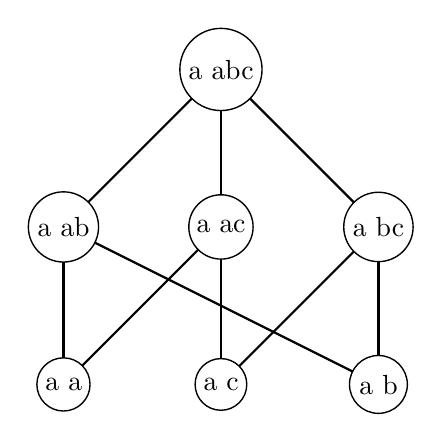
\begin{tikzpicture}
    \SetGraphUnit{2}
    \Vertex{a abc}
    \SO(a abc){a ac}
    \EA(a ac){a bc}
    \WE(a ac){a ab}
    \Edge(a abc)(a ac)
    \Edge(a abc)(a bc)
    \Edge(a abc)(a ab)
    \SO(a ac){a c}
    \EA(a c){a b}
    \WE(a c){a a}
    \Edge(a bc)(a b)
    \Edge(a bc)(a c)
    \Edge(a ac)(a c)
    \Edge(a ac)(a a)
    \Edge(a ab)(a a)
    \Edge(a ab)(a b)
  \end{tikzpicture}
  \caption{Graph of lines inferior to \reline{a~abc}.}
\end{figure}

Note that superiority is not the same relation as $\text{configurations}(A) \subseteq \text{configurations}(B)$. \reline{a abc ade} generates \reline{a b e}, while \reline{a a bcde} only generates configurations that are in \reline{a abc ade}. Yet they are incomparable in terms of superiority.

The subset of $A_{1}$ inferior to none is called the maximal form of $P_{0}$. Or one could say that the maximal form of $S$ is the Pareto front of \emph{valid} lines with respect to superiority, where valid means that a line only generates configurations that $S$ generates.

Finding the maximal form of $P_{0}$ is the most expensive part of the original Round Eliminator's algorithm. Maximization via line combination is orders of magnitude faster in practice and is resistant to some pathological inputs but it remains the most expensive part. % TODO add to abstract maybe?

% TODO explain proof that sets of configurations and lines are isomorphic

\subsection{Putting it all together}

To perform round elimination, one first finds the maximal form of the passive side. That becomes the new active side.

The new passive side is then built % TODO how exactly

Finally, to make the representation more compact, the symbols in the new alphabet are converted from subsets of the old alphabet to ordinals simply by enumerating the symbols.

\section{Coq Primer}

Before discussing my novel round elimination algorithm, I need to explain the basics of Coq because I will show the lemmas concerning its correctness as written in Coq's Vernacular. I will also give informal proofs. The actual proofs involve many boring details, which this paper does not cover. However, the Proving section will show examples of the most important proof techniques used. The full source code can be found in the project's repository\cite{source_code}.

\begin{figure}[h]
\begin{minted}{Coq}
Lemma tnth_zip n S T (a : n.-tuple T) (b : n.-tuple S) i :
  tnth (zip_tuple a b) i = (tnth a i, tnth b i).
\end{minted}
\caption{A very simple utility lemma which states that zipping two arrays of the same length and taking the $i$th item produces a tuple with the $i$th item of the first array and the $i$th item of the second list.}
\end{figure}

Lemmas in Coq are types. Constructing any value of type T proves the lemma T.

You are allowed to use values in types in order to make talking about computation convenient. This is called dependent types. Coq solves this with cumulative universes.


\section{Maximization via line combination}

\subsection{Combining lines}

My new maximization algorithm mostly consists of combining lines. Two lines can be combined by pairing up their sets and taking the union of one pair and the intersection of the rest.

The combination of two valid lines is a valid line. Proof: Let C be the combination of A and B. For each configuration c in C, Wlog. suppose the symbol that comes from the union is from A. The symbols that come from intersections are in both A and B. Thus all symbols in c are from A.

\subsection{Finding the maximal form}

A line superior to any valid line can be built by combining input lines. Thus the maximal lines can be built this way. The proof of this is less trivial and will be discussed later.

But even if the combining lines eventually produces the maximal lines, that doesn't mean it is an efficient way of finding them. However, it can be shown that if a line exists that isn't inferior to any of a set of lines then two of those lines can be combined to produce some line that isn't inferior to any of them. In other words, we can make progress by simply trying all combinations of two lines!

\section{Proving}

\subsection{Classical vs Intuitionistic Logic}

In Coq it is customary not to assume the law of excluded middle $\forall a : a \lor \lnot a$. This has little effect on the proof at hand, as it is about finite objects. For those a = b is equivalent to a == b and the latter is always true or false, as it can be computed.

\clearpage
\thesisbibliography{}

\bibliographystyle{plainnat}
\bibliography{correct_round_elimination}

%% Appendices
%% If you don't have appendices, remove \clearpage and \thesisappendix below.
\clearpage
\thesisappendix{}

\section{Esimerkki liitteestä\label{LiiteA}}

Kaavojen numerointi muodostaa liitteissä oman kokonaisuutensa:
\begin{align}
d \wedge A &= F, \label{liitekaava1}\\
d \wedge F &= 0. \label{liitekaava2}
\end{align}

\end{document}
